\documentclass{article}
\usepackage[T1]{fontenc}
\usepackage{lmodern}
\usepackage{graphicx}
\usepackage{amsmath,amssymb}
\usepackage[a4paper,margin=2cm]{geometry}
\usepackage[absolute,overlay]{textpos}
\setlength{\TPHorizModule}{1mm}
\setlength{\TPVertModule}{1mm}
\usepackage[indonesian]{babel}
\usepackage{hyperref}
\setlength{\emergencystretch}{2em}
% unit: Halaman 29

\begin{document}

% === Halaman 29 (python/native) ===

29

• Contoh: Misalkan U = 1111


 Algoritma sederhana memperoleh keystream di dalam keystream 

generator misalnya adalah sebagai berikut: 

 XOR-kan bit ke-1 dengan bit ke-4 dari empat bit sebelumnya:


111101011001000111101011...


dan akan berulang setiap 15 bit.

• Secara umum, jika panjang U adalah n bit, maka bit-bit kunci tidak akan 

berulang sampai 2n – 1 bit.

11101

1 1 1 1 0 1 0 1 1 0 0 1 0 0 0

% deskripsi: gambar native xref 141
\noindent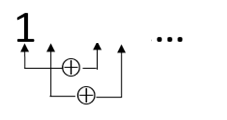
\includegraphics[width=0.85\textwidth]{../../images/python/page_029_img_01.png}

\end{document}
